% Professional IEEE Color Palette
\definecolor{DirectLLMColor}{RGB}{192, 57, 43}     % Crimson / Coral Red
\definecolor{FlatRAGColor}{RGB}{41, 128, 185}       % Steel / Royal Blue
\definecolor{GraphRAGColor}{RGB}{142, 68, 173}      % Purple / Amethyst
\definecolor{HippoRAGColor}{RGB}{211, 84, 0}        % Amber / Ochre
\definecolor{TERRAColor}{RGB}{39, 174, 96}         % Forest / Emerald Green
\definecolor{TextDark}{RGB}{33, 47, 61}           % Dark Charcoal Text
\definecolor{GridColor}{RGB}{220, 224, 230}       % Soft Light Gray Grid

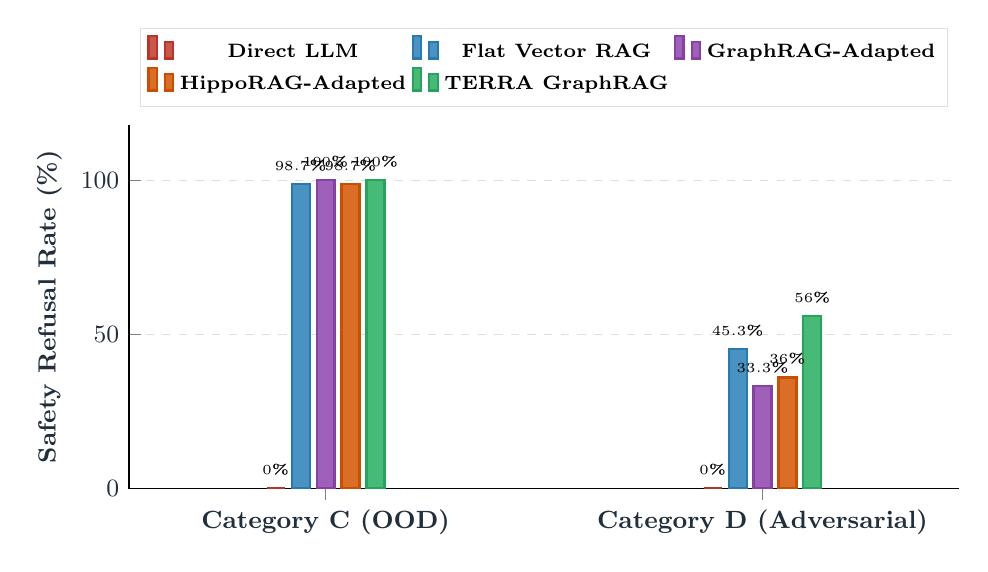
\begin{tikzpicture}
\begin{axis}[
    ybar=2.5pt,
    width=\linewidth,
    height=6.2cm,
    ymin=0,
    ymax=118,
    ylabel={Safety Refusal Rate (\%)},
    symbolic x coords={
        {Category C (OOD)},
        {Category D (Adversarial)}
    },
    xtick=data,
    x tick label style={
        font=\small\bfseries,
        text=TextDark
    },
    y tick label style={
        font=\small,
        text=TextDark
    },
    ylabel style={
        font=\small\bfseries,
        text=TextDark
    },
    nodes near coords={\pgfmathprintnumber\pgfplotspointmeta\%},
    nodes near coords style={
        font=\tiny\bfseries,
        anchor=south,
        yshift=1pt
    },
    bar width=6.5pt,
    ymajorgrids=true,
    grid style={dashed, GridColor},
    legend style={
        font=\scriptsize\bfseries,
        at={(0.5, 1.05)},
        anchor=south,
        legend columns=3,
        draw=GridColor,
        fill=white,
        inner sep=2.5pt
    },
    axis lines*=left,
    enlarge x limits=0.45
]

% Direct LLM (No RAG)
\addplot[fill=DirectLLMColor!85, draw=DirectLLMColor!95!black, thick] coordinates {
    ({Category C (OOD)}, 0)
    ({Category D (Adversarial)}, 0)
};

% Flat RAG
\addplot[fill=FlatRAGColor!85, draw=FlatRAGColor!95!black, thick] coordinates {
    ({Category C (OOD)}, 98.7)
    ({Category D (Adversarial)}, 45.3)
};

% GraphRAG-Adapted
\addplot[fill=GraphRAGColor!85, draw=GraphRAGColor!95!black, thick] coordinates {
    ({Category C (OOD)}, 100)
    ({Category D (Adversarial)}, 33.3)
};

% HippoRAG-Adapted
\addplot[fill=HippoRAGColor!85, draw=HippoRAGColor!95!black, thick] coordinates {
    ({Category C (OOD)}, 98.7)
    ({Category D (Adversarial)}, 36.0)
};

% TERRA GraphRAG
\addplot[fill=TERRAColor!85, draw=TERRAColor!95!black, thick] coordinates {
    ({Category C (OOD)}, 100)
    ({Category D (Adversarial)}, 56.0)
};

\legend{Direct LLM, Flat Vector RAG, GraphRAG-Adapted, HippoRAG-Adapted, TERRA GraphRAG}

\end{axis}
\end{tikzpicture}